\begin{solution}{Question 6}\label{ques:6}
    \begin{question}
    Prove the following stronger version of pumping lemma for CFLs: 
If $A$ is a CFL, then there is a number $k$ where if $s$ is any string in $A$ of length at least $k$ then $s$ may be divided into five pieces $s = uvxyz$, satisfying the conditions:
\begin{itemize}
    \item for each $i\geq 0$, $uv^ixy^iz \in A$
    \item $v \neq \varepsilon$, and $y \neq \varepsilon$, and
    \item $|vxy| \leq k$.
\end{itemize}
    \end{question}
    \tcblower{}
    \begin{proof}[Solution]
    We consider the proof of the original pumping lemma for CFLs. We know that for each CFL $L$ there exists a pumping length $n$ such that for a string $s = uvwxy$, $|vwx| \leq n$ and we can pump $s$ as $uv^iwx^iy$ to get a string which is in $L$. Now, if both $v \neq \epsilon$ and $x \neq \epsilon$ there is no need to prove further and we are done.\par
    Now, in the original proof, we had considered a parse tree of height $h + 1$ such that $h = |V|$ (so that we have at least one non-terminal repeating). Now, we consider a parse tree of height $2h + 1$. We will have at least one non-terminal repeating thrice in this case. Now, we have two possibilities:
    \begin{enumerate}
        \item \textbf{The same non terminals do not appear consecutively:} Let $A$ be the non-terminal repeating thrice. We ignore the occurrence in the middle. Since $A_{first}$ and $A_{last}$ are not consecutive, on observing the parse tree, it is clearly visible that neither $v = \epsilon$ nor $y = \epsilon$. Hence the stronger pumping lemma holds and is valid.
        \begin{figure}[H]
            \centering
            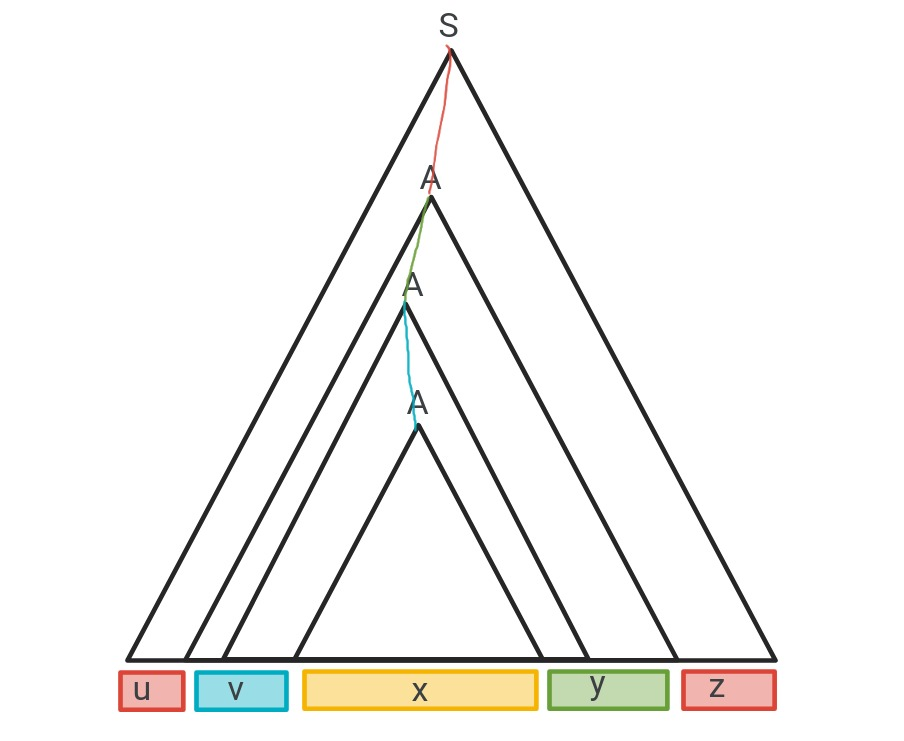
\includegraphics[width=0.5\textwidth]{case 1.jpeg}
            \caption{Parse tree for case 1}
        \end{figure}
        \item \textbf{The non-terminals appear consecutively:} Let $A$ be the non-terminal repeating thrice. For this case, we pump the string differently. We repeat the production which is present between the first two (consecutive) occurrences of $A$ an arbitrary number of times (possibly even zero). We also repeat the production which is present between the last two (consecutive) occurrences of $A$ an arbitrary number of times (possibly even zero). Therefore, the string we get is $uvw^ix^jy$. We take $i = j$ to get $(uv)w^i(\epsilon)x^iy$. This is equivalent to $u'(v')^ix'(y')^iz'$ where $u' = uv, v' = w, x' = \epsilon, y' = x, z' = y$.
        \begin{figure}[H]
            \centering
            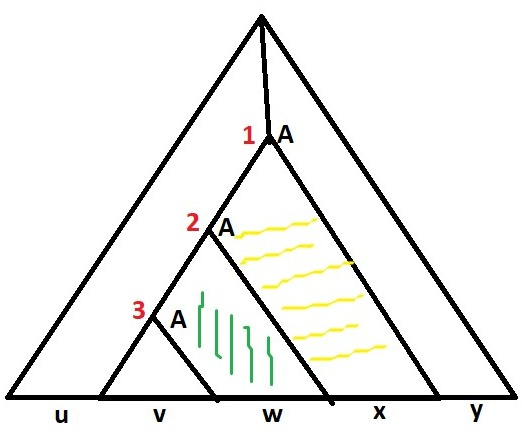
\includegraphics[width=0.5\textwidth]{case 2.jpeg}
            \caption{Parse tree for case 2}
        \end{figure}
    \end{enumerate}
    Therefore, we have shown the stronger version of pumping lemma to hold for both cases. Therefore, the stronger version of pumping lemma is proven for CFLs.
    \end{proof}
\end{solution}
